\chapter{Requirement Analysis}
This chapter includes analysis of the requirements of the system based on the problem statement described in the previous chapter. Furthermore, the main goal of the software as well as other specifications will be analyzed.

\section{Goal}
The goal of this research project is to build a functional prototype of a mobile application that monitors users' health and activity by observing users' heart rate. To observe one's heart rate, the application will be establish connection to a heart rate sensor via bluetooth low energy.
With the help of bluetooth low energy connection, the sensor is able to broadcast heart rate data to the application while consuming minimal energy.
The retrieved data will be stored in local database instead of cloud services or wearable devices to ensure data privacy. The user will also be given full control over their data, allowing them to modify or delete their data according to their will at anytime.
The retrieved data can be accessed later for visualization purposes as long as it is available. Furthermore, the application should be able to calculate users' energy expenditure during their exercise based on their heart rate, age, gender, weight, duration of exercise.

\section{State of the Art}
Health monitoring using wearable devices has gained immense popularity, enabling individuals to conveniently monitor their health and fitness. Bluetooth low energy (BLE) plays an important role in establishing connection between wearable device, which acts as a sensor, and the application. 
BLE offers real-time data exchange while consuming low power, which allows for long-term deployment without the need of frequent battery change. \cite{strey2013ble}
Existing health and activity monitor applications utilizing BLE offer a range of features and functionalities such as heart rate, calories burned, sleep patterns.

Nevertheless, as mentioned earlier, the challenges remain in maintaining a straightforward application and ensuring users' privacy. The aim in this research project is to explore the possibilities of improving health and wellbeing of the user by providing real-time data on their heart rate while providing users full control over their own data.
By addressing these challenges, this research project intends to develop a prototype of a more user- and privacy-friendly health activity monitor application using BLE.
\newpage

\section{Requirements}
\label{chap:requirements}
In this chapter, the requirements of the application is listed by identifying and analyzing the use cases from the research project's goals and priorities.

\subsection{Use Cases}
A use case diagram is created to provide a clearer understanding of how the system works and the various usage scenarios. It offers a clear and straightforward visualization that aligns with the goal of the research project.
\begin{figure}[H]
    \centering
    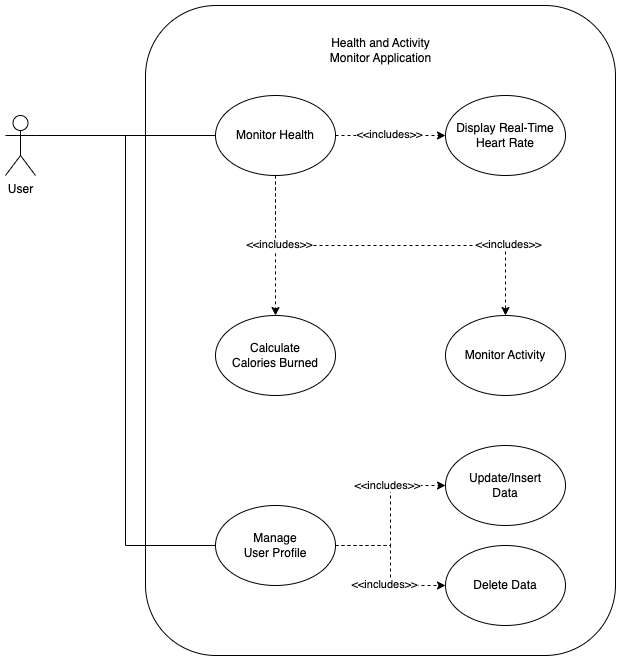
\includegraphics[width=1\textwidth]{diagrams/usecase.drawio.png}
    \caption{Use case diagram of the health and activity monitor application}
    \label{fig:use_cases}
\end{figure}
\newpage
The use case diagram provides visual presentation of the primary system functionalities and identifies the actor that interacts with the system.
The system includes several use cases to provide a comprehensive experience for monitoring health and activity while ensuring user's data privacy.

The primary use case, "Monitor Health", allows users to track important health indicators such as heart rate, calories burned, and current activity. It consists of three sub-use cases: "Display Real-Time Heart Rate", which shows the user's live heart rate on the application's interface; "Calculate Calories Burned", which calculates the number of calories burned in an exercise based on the user's heart rate;  "Monitor Activity", which observes the user's ongoing physical activity. In addition, the system includes "Manage User Profile" use case, which handles user profile management and data manipulation. Users can update or insert or delete data anytime using the respective sub-use cases. By integrating these use cases, the system effectively monitor health metrics and allows user to conveniently manage their data.

\subsection{User Stories}
According to the use cases visualized on \autoref{fig:use_cases}, the following user stories can be determined:

\begin{itemize}[label={},leftmargin=*]
    \item \textbf{Display Real-Time Heart Rate}
      \begin{itemize}[label={},leftmargin=*]
        \item As a health-oriented user, I want the application to show my live heart rate so that I can monitor my cardiovascular activity.
      \end{itemize}

    \item \textbf{Track and Monitor Current Activity}
      \begin{itemize}[label={},leftmargin=*]
        \item As an physically active individuals, I want the application to track and display my current activity so that I can keep track of my progress and make adjustments to my physical activities.
      \end{itemize}

    \item \textbf{Calculate Calories Burned}
      \begin{itemize}[label={},leftmargin=*]
        \item As a fitness enthusiast, I want the application to calculate and display the number of calories burned based in my exercises. This allows me to keep track of my progress and make adjustments to my exercises.
      \end{itemize}  

    \item \textbf{Profile Management}
      \begin{itemize}[label={},leftmargin=*]
        \item As a user of the application who is concerned about data privacy, I want to be able to manage my user profile easily. This includes updating or adding new information to my profile and create a new profile. I also want the ability to delete my data anytime. This allows me to have full control over my data.
      \end{itemize}
  \end{itemize}


\subsection{Application Quality Standard}
The evaluation of the system developed for this research project is guided by the core application quality standard outlined in Android Documentation \autocite{androidqualityguidelines}. These quality standards provide core foundation for assessing the quality of the application. To facilitate the evaluation a set of criteria is derived from the core application quality standard described outlined in Android Documentation \autocite{androidqualityguidelines}. The table below shows the criteria, along with the sub-characteristic as well as its relevance to the research project. These criteria will be reviewed during the evaluation process to assess the quality of the application developed in this research project.
\label{tab::qualitystandard}

\begin{longtable}{p{0.2\textwidth} p{0.1\textwidth} p{0.5\textwidth} p{0.2\textwidth}}

    \caption{Core application quality standard based on Android Documentation \autocite{androidqualityguidelines} and its importance}\\

        \hline
        \textbf{Area} & \textbf{ID} & \textbf{Description} & \textbf{Relevance} \\
        \hline
        Navigation & VX-N1 & The app supports standard Back button navigation and does not make use of any custom, on-screen "Back button" prompts. & less important \\
         & VX-N2 & The app supports gesture navigation for going back / going to the home screen. & less important \\
         & VX-N3 & The app correctly preserves and restores user or app state. & important \\
  
        UI and Graphics & VX-U1 & The app supports both landscape and portrait orientations (if possible) and folding / unfolding. & important \\
         & VX-U2 & The app uses the whole screen in both orientations and does not letterbox to account for orientation changes, including folding and unfolding. & not important \\
         & VX-U3 & The app correctly handles rapid transitions between display orientations and device folding / unfolding without rendering problems or losing state. & less important \\
  
        Visual quality & VX-V1 & The app displays graphics, text, images, and other UI elements without noticeable distortion, blurring, or pixelation. The app should use vector drawables where possible. & less important \\
         & VX-V2 & The app displays text and text blocks in an acceptable manner for each of the app's supported languages. & important \\
         & VX-V3 & The app's content, and all web contents referred to by the app, support dark theme. & not important \\
        Accessibility & VX-A1 & Touch targets should be at least 48dp in size. & less important \\
         & VX-A2 & The app's text and foreground content should maintain a high enough color contrast ratio with its background. & important \\
         & VX-A3 & Describe each UI element, except for TextView, using contentDescription. & not important \\
  
        Background Service & FN-B1 & The app avoids running unnecessarily long services in the background. To ensure the smooth running of the user's device, the system applies various restrictions on background services. & important\\

        Stability & PS-S1 & The app does not crash or block the UI thread causing ANR ("Android Not Responding") errors.  & very important\\

        Performance & PS-P1 & The app loads quickly or provides onscreen feedback to the user (a progress indicator or similar cue) if the app takes longer than two seconds to load. & important\\
        & PS-P2 & Apps should render frames every 16ms to achieve 60 frames per second. Developers can use the Profile HWUI rendering option in testing. If there are issues, tools are available to help diagnose slow rendering. & less important\\
        & PS-P3 & With StrictMode enabled (see StrictMode Testing, below), no red flashes (performance warnings from StrictMode) are visible when testing the app. Any red flashes indicate bad behaviors regarding storage, network access, or memory leaks.  & less important\\
        
        Permissions & SC-P1 & The app requests only the absolute minimum number of permissions that it needs to support its use case at hand. & important \\
        & SC-P2 & The app requests permission to access sensitive data (such as SMS, Call Log, or Location) or services that cost money (such as Dialer or SMS) only when directly related to the core use cases of the app. & important \\
        & SC-P3 & The app requests runtime permissions in context, when the functionality is requested, rather than upfront during app startup. & less important\\
        & SC-P4 & The app clearly conveys why certain permissions are needed or follows the recommended flow to explain why it needs a permission. &  important \\
        & SC-P5 & The app should gracefully degrade when users deny or revoke a permission. The app should not prevent the user from accessing the app altogether. & important\\
        
        Data \& Files & SC-DF1 & All sensitive data is stored in the app's internal storage. & important\\
         & SC-DF2 & No personal or sensitive user data is logged to the system log or an app-specific log. & important\\
         & SC-DF3 & The app does not use any non-resettable hardware IDs, such as the IMEI, for identification purposes. & less important\\

        
        \hline
\end{longtable}

